\section{Evaluation Results, Analysis and Discussion.}

\subsection{Performance Comparison Across Memory-Enabled Systems}
Table~\ref{tab:results} reports \Fone, \Bone~and \Judge~scores for our two architectures—\mem~and \memp~—against a suite of competitive baselines, as mentioned in Section \ref{sec:experiment_setup}, on single‑hop, multi‑hop, open‑domain, and temporal questions. Overall, both of our models set new state‑of‑the‑art marks in all the three evaluation metrics for most question types.


\paragraph{Single-Hop Question Performance} Single‑hop queries involve locating a single factual span contained within one dialogue turn. Leveraging its dense memories in natural language text, \mem~secures the strongest results:\Fone=38.72, \Bone=27.13, and \Judge=67.13. Augmenting the natural language memories with graph memory (\memp) yields marginal performance drop compared to \mem, indicating that relational structure provides limited utility when the retrieval target occupies a single turn. Among the existing baselines, the full‑context \texttt{OpenAI} run attains the next‑best \Judge\ score, reflecting the benefits of retaining the entire conversation in context, while LangMem and Zep both score around 8\% relatively less against our models on \Judge~score. Previous \texttt{LOCOMO} benchmarks such as A-mem lag by more than 25 points in \Judge, underscoring the necessity of fine‑grained, structured memory indexing even for simple retrieval tasks.

\paragraph{Multi-Hop Question Performance}
Multi-hop queries require synthesizing information dispersed across multiple conversation sessions, posing significant challenges in memory integration and retrieval. \mem~clearly outperforms other methods with an \Fone~score of 28.64 and a \Judge~score of 51.15, reflecting its capability to efficiently retrieve and integrate disparate information stored across sessions. Interestingly, the addition of graph memory in \memp~does not provide performance gains here, indicating potential inefficiencies or redundancies in structured graph representations for complex integrative tasks compared to dense natural language memory alone. Baselines like LangMem show competitive performances, but their scores substantially trail those of \mem, emphasizing the advantage of our refined memory indexing and retrieval mechanisms for complex query processing.

\paragraph{Open-Domain Performance}
In open-domain settings, the baseline Zep achieves the highest \Fone\ (49.56) and \Judge\ (76.60) scores, edging out our methods by a narrow margin.  In particular, Zep’s \Judge\ score of 76.60 surpasses \memp’s 75.71 by just 0.89 percentage points and outperforms \mem’s 72.93 by 3.67 points, highlighting a consistent, if slight, advantage in integrating conversational memory with external knowledge. \memp remains a strong runner-up, with a \Judge\ of 75.71 reflecting high factual retrieval precision, while \mem~follows with 72.93, demonstrating robust coherence. These results underscore that although structured relational memories (as in \mem\ and \memp) substantially improve open-domain retrieval, Zep maintains a small but meaningful lead.


\paragraph{Temporal Reasoning Performance}
Temporal reasoning tasks hinge on accurate modeling of event sequences, their relative ordering, and durations within conversational history. Our architectures demonstrate substantial improvements across all metrics, with \memp~achieving the highest \Fone (51.55) and \Judge~(58.13), suggesting that structured relational representations in addition to natural language memories significantly aid in temporally grounded judgments. Notably, the base variant, \mem, also provide a decent \Judge~score (55.51), suggesting that natural language alone can aid in temporally grounded judgments. 
Among baselines, OpenAI notably underperforms, with scores below 15\%, primarily due to missing timestamps in most generated memories despite explicit prompting in the OpenAI ChatGPT to extract memories with timestamps. Other baselines such as A-Mem achieve respectable results, yet our models clearly advance the state-of-the-art, emphasizing the critical advantage of accurately leveraging both natural language contextualization and structured graph representations for temporal reasoning.


\subsection{Cross-Category Analysis}
The comprehensive evaluation across diverse question categories reveals that our proposed architectures, \mem~and \memp, consistently achieve superior performance compared to baseline systems. For single-hop queries, \mem~demonstrates particularly strong performance, benefiting from its efficient dense natural language memory structure. Although graph-based representations in \memp~slightly lag behind in lexical overlap metrics for these simpler queries, they significantly enhance semantic coherence, as demonstrated by competitive \Judge~scores. This indicates that graph structures are more beneficial in scenarios involving nuanced relational context rather than straightforward retrieval. For multi-hop questions, \mem~exhibits clear advantages by effectively synthesizing dispersed information across multiple sessions, confirming that natural language memories provide sufficient representational richness for these integrative tasks. Surprisingly, the expected relational advantages of \memp~do not translate into better outcomes here, suggesting potential overhead or redundancy when navigating more intricate graph structures in multi-step reasoning scenarios.

\begin{table}[!t]
\centering
\caption{Performance comparison of various baselines with proposed methods. Latency measurements show p50 (median) and p95 (95th percentile) values in seconds for both search time (time taken to fetch memories/chunks) and total time (time to generate the complete response). Overall LLM-as-a-Judge score ($\mathrm{J}$) represents the quality metric of the generated responses on the entire \texttt{LOCOMO} dataset.}
\begin{tabular*}{\textwidth}{@{\extracolsep{\fill}}lcccccccc@{}}
\toprule
\multirow{3}{*}{\textit{\textbf{Method}}} & \multicolumn{2}{c}{} & \multicolumn{4}{c}{\textit{\textbf{Latency (seconds)}}} & \multirow{3}{*}{\begin{tabular}[c]{@{}c@{}}\textit{\textbf{Overall}} \\$\mathrm{J}$\end{tabular}} \\
\cmidrule(lr){4-7}
 & \multicolumn{2}{c}{} & \multicolumn{2}{c}{\textbf{Search}} & \multicolumn{2}{c}{\textbf{Total}} & \\
\cmidrule(lr){4-5} \cmidrule(lr){6-7}
& \textbf{K}
& \begin{tabular}{@{}c@{}}
    \textbf{chunk size} / \\
    \textbf{memory tokens}
  \end{tabular}
& \textbf{p50} & \textbf{p95}
& \textbf{p50} & \textbf{p95}
& \\
\midrule
\multirow{14}{*}{RAG} & \multirow{7}{*}{1} & 128 & 0.281  & 0.823 & 0.774 & 1.825 & 47.77 $\pm$ 0.23\% \\
 &  & 256 & 0.251 & 0.710 & 0.745 & 1.628 & 50.15 $\pm$ 0.16\% \\
 &  & 512 & 0.240 & 0.639 & 0.772 & 1.710 & 46.05 $\pm$ 0.14\% \\
 &  & 1024 & 0.240 & 0.723 & 0.821 & 1.957 & 40.74  $\pm$ 0.17\% \\
 &  & 2048 & 0.255 & 0.752 & 0.996 & 2.182 & 37.93 $\pm$ 0.12\% \\
 &  & 4096 & 0.254 & 0.719 & 1.093 & 2.711 & 36.84 $\pm$ 0.17\% \\
 &  & 8192 & 0.279 & 0.838 & 1.396 & 4.416 & 44.53 $\pm$ 0.13\% \\
\cmidrule{2-8}
 & \multirow{7}{*}{2} & 128 & 0.267 & 0.624 & 0.766 & 1.829 & 59.56 $\pm$ 0.19\% \\
 &  & 256 & 0.255  & 0.699 & 0.802 & 1.907 & 60.97 $\pm$ 0.20\% \\
 &  & 512 & 0.247 & 0.746 & 0.829 & 1.729 & 58.19 $\pm$ 0.18\% \\
 &  & 1024 & 0.238 & 0.702 & 0.860 & 1.850 & 50.68 $\pm$ 0.13\% \\
 &  & 2048 & 0.261 & 0.829 & 1.101 & 2.791 & 48.57 $\pm$ 0.22\% \\
 &  & 4096 & 0.266 & 0.944 & 1.451 & 4.822 & 51.79 $\pm$ 0.15\% \\
 &  & 8192 & 0.288 & 1.124 & 2.312 & 9.942 & 60.53 $\pm$ 0.16\% \\
\midrule
Full-context &  & 26031 & - & - & 9.870 & 17.117 & \textbf{72.90 $\pm$ 0.19\%} \\
\midrule
A-Mem &  & 2520 & 0.668 & 1.485 & 1.410 & 4.374 & 48.38 $\pm$ 0.15\% \\
LangMem &  & \textbf{127} & 17.99 & 59.82 & 18.53 & 60.40 & 58.10 $\pm$ 0.21\% \\
Zep &  & 3911 & 0.513 & 0.778 & 1.292 & 2.926 & 65.99 $\pm$ 0.16\% \\
OpenAI &  & 4437 & - & - & 0.466 & 0.889 & 52.90 $\pm$ 0.14\% \\ 
\midrule
\mem &  & 1764 & \textbf{0.148} & \textbf{0.200} & \textbf{0.708} & \textbf{1.440} & 66.88 $\pm$ 0.15\% \\
\memp &  & 3616 & 0.476 & 0.657 & 1.091 & 2.590 & 68.44 $\pm$ 0.17\% \\
\bottomrule
\end{tabular*}
\label{tab:latency_comparison}
\end{table}


In temporal reasoning, \memp~substantially outperforms other methods, validating that structured relational graphs excel in capturing chronological relationships and event sequences. The presence of explicit relational context significantly enhances \memp's temporal coherence, outperforming \mem's dense memory storage and highlighting the importance of precise relational representations when tracking temporally sensitive information. Open-domain performance further reinforces the value of relational modeling. \memp, benefiting from the relational clarity of graph-based memory, closely competes with the top-performing baseline (Zep). This competitive result underscores \memp's robustness in integrating external knowledge through relational clarity, suggesting an optimal synergy between structured memory and open-domain information synthesis.

Overall, our analysis indicates complementary strengths of \mem~and \memp~across various task demands: dense, natural-language-based memory offers significant efficiency for simpler queries, while explicit relational modeling becomes essential for tasks demanding nuanced temporal and contextual integration. 
These findings reinforce the importance of adaptable memory structures tailored to specific reasoning contexts in AI agent deployments.

\begin{figure}[!t]
    \centering
    \begin{subfigure}{\textwidth}
        \centering
        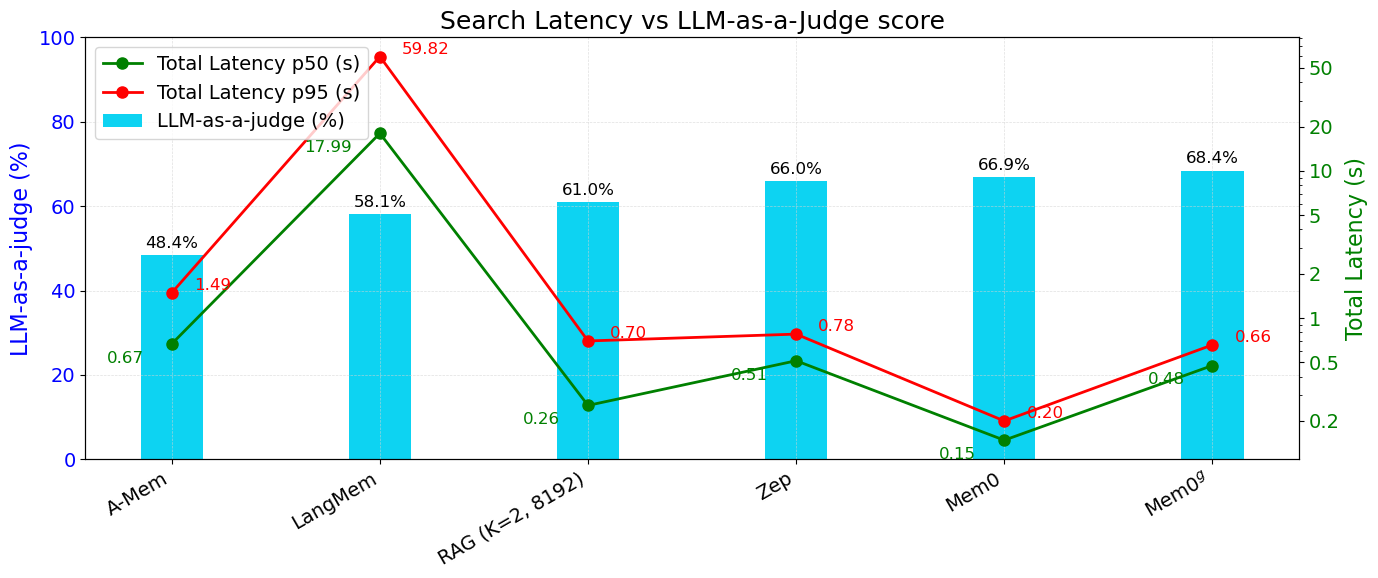
\includegraphics[width=0.97\textwidth]{figures/latency_search.png}
        \caption{Comparison of \emph{search} latency at p50 (median) and p95 (95th percentile) across different memory methods (\mem, \memp, best RAG variant, Zep, LangMem, and A-Mem). The bar heights represent \Judge~scores (left axis), while the line plots show search latency in seconds (right axis scaled in log).}
        \label{fig:latency_search}
    \end{subfigure}
    \begin{subfigure}{\textwidth}
        \centering
        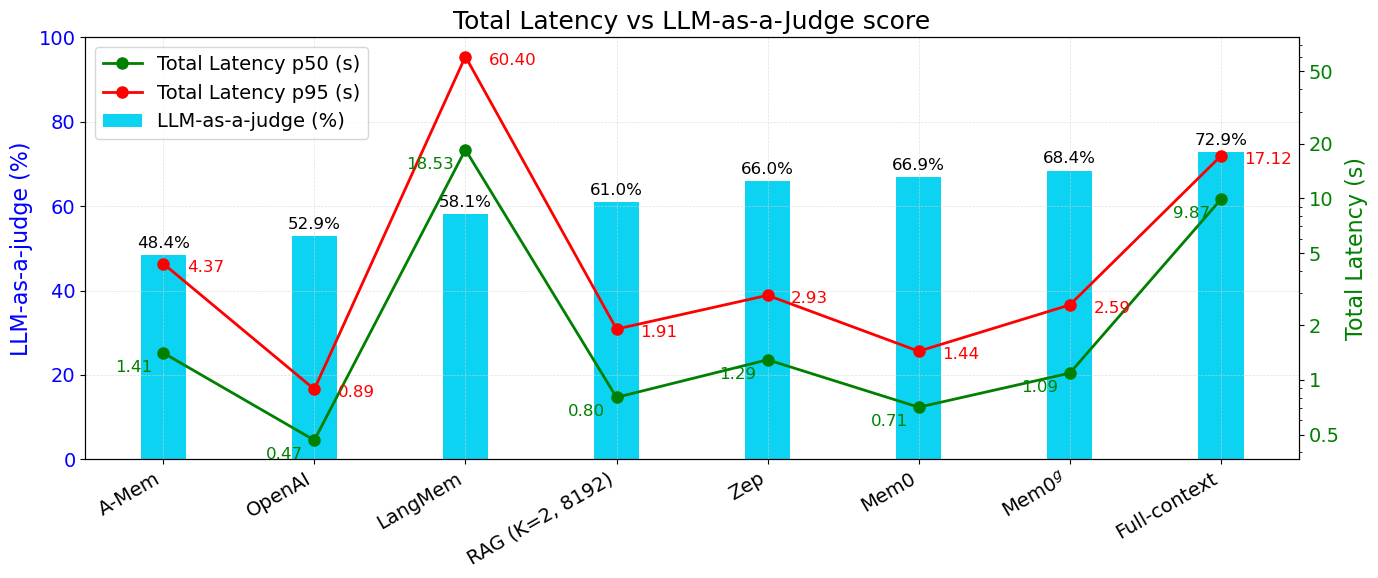
\includegraphics[width=0.97\textwidth]{figures/latency_total.png}
        \caption{Comparison of \emph{total response} latency at p50 and p95  across different memory methods (\mem, \memp, best RAG variant, Zep, LangMem, OpenAI, full-context, and A-Mem). The bar heights represent \Judge~scores (left axis), and the line plots capture end-to-end latency in seconds (right axis scaled in log).}
        \label{fig:latency_total}
    \end{subfigure}
    \caption{%
    \textbf{Latency Analysis of Different Memory Approaches.} 
    These subfigures illustrate the \Judge~scores and latency comparison of various selected methods from Table \ref{tab:latency_comparison}.
    Subfigure~(a) highlights the \emph{search/retrieval} latency prior to answer generation, while Subfigure~(b) shows the \emph{total} latency (including LLM inference).
    Both plots overlay each method’s \Judge~score for a holistic view of their accuracy and efficiency.
    }
    \label{fig:latency_combined}
\end{figure}


\subsection{Performance Comparison of \mem~and \memp~Against RAG Approaches and Full-Context Model}
Comparisons in Table \ref{tab:latency_comparison}, focusing on the `Overall \Judge' column, reveal that both \mem~and \memp~consistently outperform all RAG configurations, which vary chunk sizes (128–8192 tokens) and retrieve either one ($k$=1) or two ($k$=2) chunks. Even the strongest RAG approach peaks at around 61\% in the \Judge~metric, whereas \mem~reaches 67\%—about a 10\% relative improvement—and \memp~reaches over 68\%, achieving around a 12\% relative gain. These advances underscore the advantage of capturing only the most salient facts in memory, rather than retrieving large chunk of original text. By converting the conversation history into concise, structured representations, \mem~and \memp~mitigate noise and surface more precise cues to the LLM, leading to better answers as evaluated by an external LLM (\Judge).

Despite these improvements, a full-context method that ingests a chunk of roughly 26,000 tokens still achieves the highest \Judge~score (approximately 73\%). However, as shown in Figure \ref{fig:latency_total}, it also incurs a very high total p95 latency—around 17 seconds—since the model must read the entire conversation on every query. By contrast, \mem~and \memp~significantly reduce token usage and thus achieve lower p95 latencies of around 1.44 seconds (a 92\% reduction) and 2.6 seconds (a 85\% reduction), respectively over full-context approach. Although the full-context approach can provide a slight accuracy edge, the memory-based systems offer a more practical trade-off, maintaining near-competitive quality while imposing only a fraction of the token and latency cost. 
As conversation length increases, full-context approaches suffer from exponential growth in computational overhead (evident in Table \ref{tab:latency_comparison} where total p95 latency increases significantly with larger $k$ values or chunk sizes). This increase in input chunks leads to longer response times and higher token consumption costs. In contrast, memory-focused approaches like \mem~and \memp~maintain consistent performance regardless of conversation length, making them substantially more viable for production-scale deployments where efficiency and responsiveness are critical.



\subsection{Latency Analysis}
Table \ref{tab:latency_comparison} provides a comprehensive performance comparison of various retrieval and memory methodologies, presenting median (p50) and tail (p95) latencies for both the search phase and total response generation across the \texttt{LOCOMO} dataset. Our analysis reveals distinct performance patterns governed by architectural choices. Memory-centric architectures demonstrate different performance characteristics. A-Mem, despite its larger memory store, incurs substantial search overhead (p50: 0.668s), resulting in total median latencies of 1.410s. LangMem exhibits even higher search latencies (p50: 17.99s, p95: 59.82s), rendering it impractical for interactive applications. Zep achieves moderate performance (p50 total: 1.292s).
The full-context baseline, which processes the entire conversation history without retrieval, fundamentally differs from retrieval-based approaches. By passing the entire conversation context (26000 tokens) directly to the LLM, it eliminates search overhead but incurs extreme total latencies (p50: 9.870s, p95: 17.117s). Similarly, the OpenAI implementation does not perform memory search, as it processes manually extracted memories from their playground. While this approach achieves impressive response generation times (p50: 0.466s, p95: 0.889s), it requires pre-extraction of relevant context, which is not reflected in the reported metrics.

Our proposed \mem~approach achieves the lowest search latency among all methods (p50: 0.148s, p95: 0.200s) as illustrated in Figure \ref{fig:latency_search}. This efficiency stems from our selective memory retrieval mechanism and infra improvements that dynamically identifies and retrieves only the most salient information rather than fixed-size chunks. Consequently, \mem~maintains the lowest total median latency (0.708s) with remarkably contained p95 values (1.440s), making it particularly suitable for latency-sensitive applications such as interactive AI agents. The graph-enhanced \memp~variant introduces additional relational modeling capabilities at a moderate latency cost, with search times (0.476s) still outperforming all existing memory solutions and baselines. 
Despite this increase, \memp~maintains competitive total latencies (p50: 1.091s, p95: 2.590s) while achieving the highest \Judge~score (68.44\%) across all methods—trailing only the computationally prohibitive full-context approach.
This performance profile demonstrates our methods' ability to balance response quality and computational efficiency, offering a compelling solution for production AI agents where both factors are critical constraints.


\subsection{Memory System Overhead: Token Analysis and Construction Time}
We measure the average token budget required to materialise each system's long‑term memory store.
\mem~encodes complete dialogue turns in a natural language representation and therefore occupies only \textbf{7k} tokens per conversation on an average. Where as \memp~roughly doubles the footprint to \textbf{14k} tokens, due to the introduction of graph memories which includes nodes and corresponding relationships. In stark contrast, Zep's memory graph consumes in excess of \textbf{600k} tokens. The inflation arises from Zep's design choice to cache a full abstractive summary at every node while also storing facts on the connecting edges, leading to extensive redundancy across the graph. For perspective, supplying the \emph{entire} raw conversation context to the language model—without any memory abstraction—amounts to roughly \textbf{26k} tokens on average, 20 times less relative to Zep's graph.
Beyond token inefficiency, our experiments revealed significant operational bottlenecks with Zep. After adding memories to Zep's system, we observed that immediate memory retrieval attempts often failed to answer our queries correctly. Interestingly, re-running identical searches after a delay of several hours yielded considerably better results. This latency suggests that Zep's graph construction involves multiple asynchronous LLM calls and extensive background processing, making the memory system impractical for real-time applications. In contrast, \mem~graph construction completes in under a minute even in worst-case scenarios, allowing users to immediately leverage newly added memories for query responses.

These findings highlight that Zep not only replicates identical knowledge fragments across multiple nodes, but also introduces significant operational delays. Our architectures—\mem~and \memp—preserve the same information at a fraction of the token cost and with substantially faster memory availability, offering a more memory‑efficient and operationally responsive representation.